\chapter{{Implementacja programowa systemu}}
\label{chapter:implementacja}
\thispagestyle{empty}

W niniejszym rozdziale pokazane zostały etapy budowania aplikacji. Poszczególne części rozdziału zawierają kolejno diagramy, opis budowy aplikacji oraz zrzuty ekrany gotowej aplikacji z podziałem na funkcjonalności.

\section{{Diagram klas}}

\begin{figure}[h!]
  \centering
  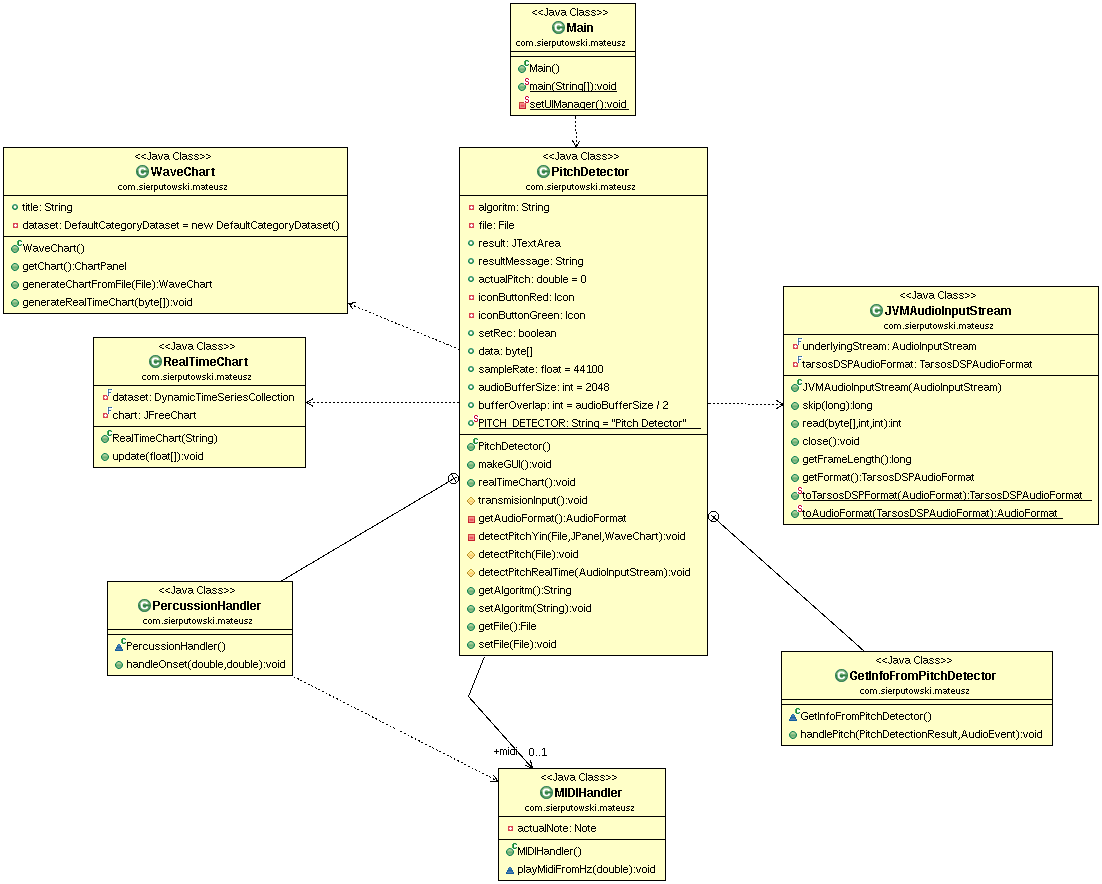
\includegraphics[width=1\linewidth]{rys/diagram1}
  \caption{Diagram klas.}
  \label{fig:schemat}
\end{figure}

Powyższy diagram przedstawia klasy użyte w tej pracy inżynierskiej. Główną klasą aplikacji jest klasa PitchDetector. Nazwa tej klasy odzwierciedla również nazwę aplikacji. Jest to główna klasa zawierająca interface graficzny użytkownika. Zawiera również obiekty obsługujące większość funkcjonalności aplikacji. Zawiera również niezbędne do poprawnego działania aplikacji ustawienia domyślne. 


Kolejną klasą zawartą w diagramie jest klasa WaveChart. Klasa ta jest odpowiedzialna za generowanie wykresów. Jest ograniczona jedynie do tworzenia wykresów na podstawie plików wczytanych z dysku. Aby rozszerzyć funkcjonalność, została również stworzona klasa odpowiedzialna za generowanie wykresów w czasie rzeczywistym z przekazywanego strumienia danych o nazwie RealTimeChart. Do obsługi strumieni danych oprócz standardowych bibliotek Javy została wykorzystana klasa JVMAudioInputStream. W celu realizacji jednego z dwóch głównych celów aplikacji zostały stworzone dwie klasy, kolejno GetInfoFromPitchDetector oraz PercussionHandler. Pierwsza z nich jest odpowiedzialna za wykrywanie tonów, druga zaś wykrywa rozpoczęcie trwania tonu w czasie. Aby zrealizować drugi cel aplikacji, użyta została klasa MIDIHandler, która zawiera obsługę protokołu MIDI.


\section{{Opis działania aplikacji}}

W tym rozdziale zostanie omówione działanie aplikacji. Sposób poruszania się po niej oraz obsługi.


Na rysunku zamieszczono zrzuty ekranu ukończonej aplikacji.

\begin{figure}[h!]
  \centering
  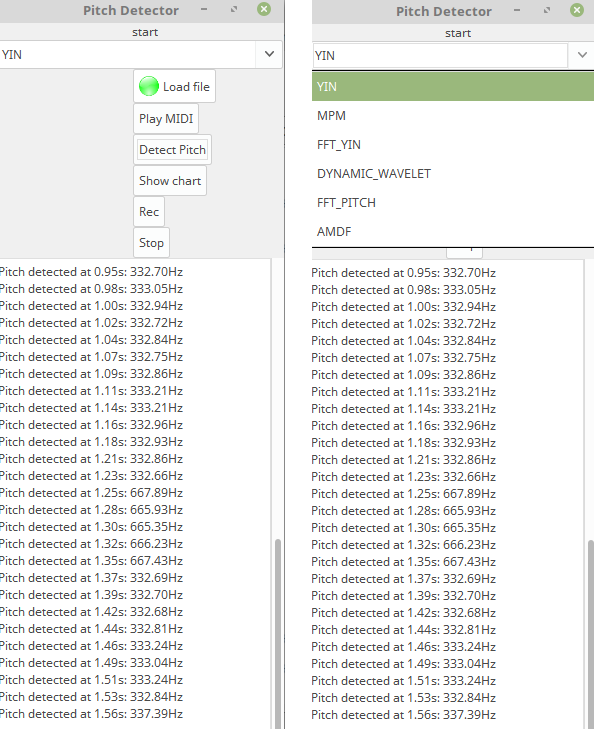
\includegraphics[width=0.5\linewidth]{rys/zrzut1}
  \caption{Zrzut ekranu aplikacjii.}
  \label{fig:schemat}
\end{figure}


Na zrzucie ekranu został przedstawiony interfejs graficzny użytkownika. Do wykonania GUI został wykorzystany pakiet Swing. W górnej części aplikacji znajdują się przyciski funkcjonalne, poniżej został wykorzystany komponent Text Area, który służy do wyświetlania informacji generowanych przez program. Został przedstawiony sposób wyboru algorytmu, który ma posłużyć do wykrywania tonu. Wykorzystany został również mechanizm obsługujący ładowanie plików z dysku.